\subsection{Panning and Zooming}
Pan and zoom are very useful tools in eCAD. The zoom tool is invaluable when you need to move up close to an entity to work on it. This is especially true when the area is very small, or several lines drawn close together. As you will see in a moment, there are several ways to use zoom. Pan allows you to move the drawing up, down, right, or left. This is especially useful if your drawing is large. Pan and zoom are accomplished by two methods. Either from the menu or using cursor.
\begin{enumerate}
\item \textbf{From Menu}
\begin{itemize}
\item Zoom In: Go to View then click Zoom In to zoom.
\item Zoom Out: Go to View then Click Zoom Out to zoom.
\item Panning: Go to view then click Panning, hand cursor will appear now you can move the screen as you want to do that.
\end{itemize}
\item \textbf{Using cursor}:
Zooming can be achieved by mouse wheel scrolling. By default, wheel scrolling triggers zooming-in/out respectively.
\end{enumerate}

\subsection{Toggling Visibility}
There are various which we can set according to our requirement. Like grid, scripting console, command console, status bar, tool bar etc. It all depends upon user need how user want to see the screen. 
\begin{enumerate}
\item \textbf{Grid}:
\begin{figure}[h!]
\centering
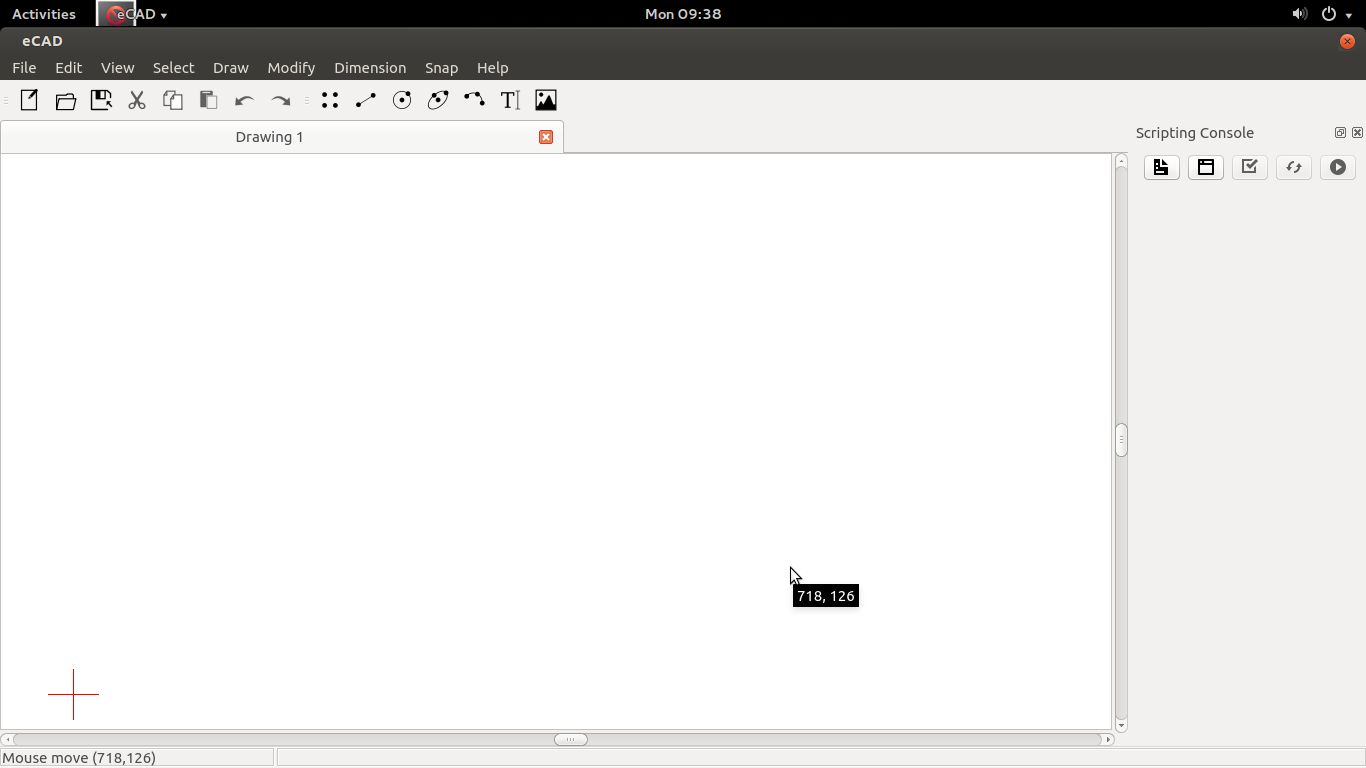
\includegraphics[width=0.7\textwidth]{images/togglegrig.png}\\
Go to View the uncheck the grid Grid will not be visible.
\end{figure}
\newpage
\item \textbf{Scripting Console}:
\begin{figure}[h!]
\centering
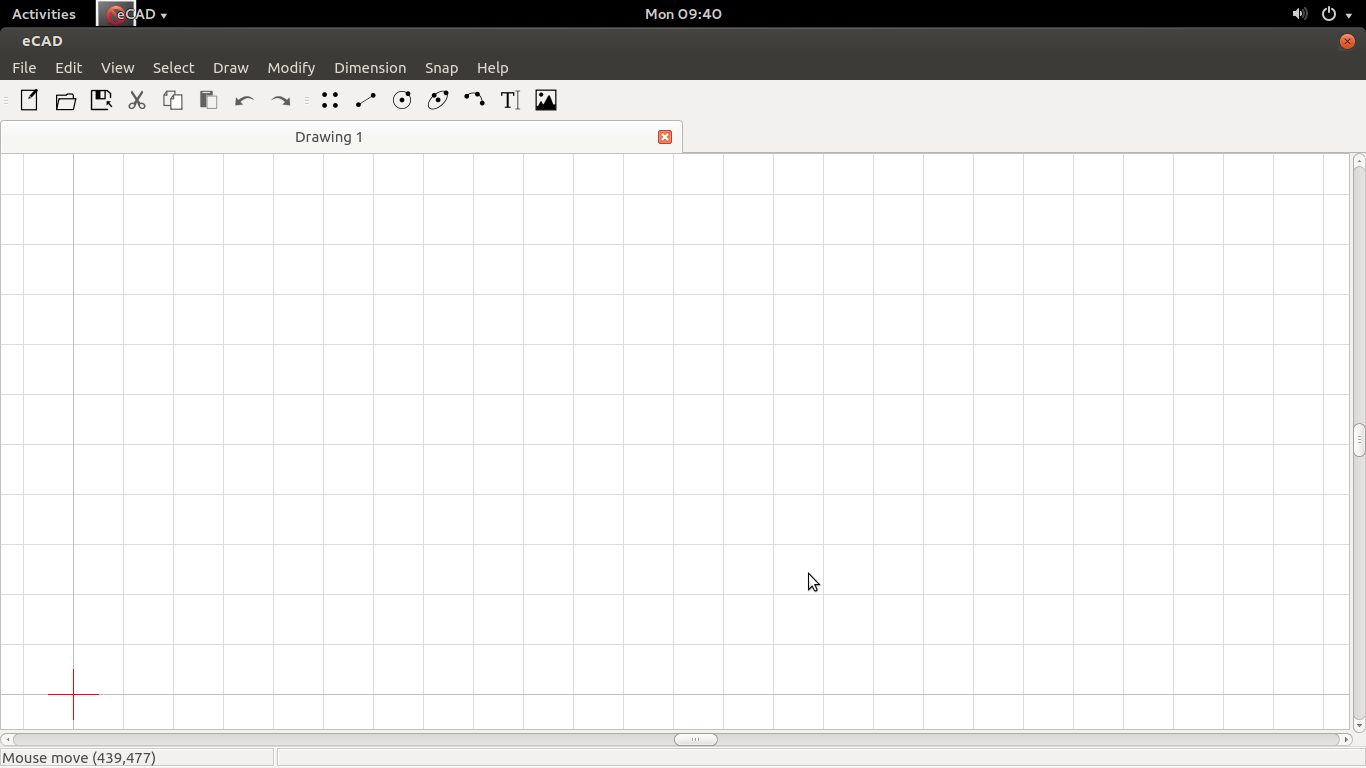
\includegraphics[width=0.7\textwidth]{images/togglescripting.png}\\
Go to View then Toolbars and uncheck the scripting. Scripting widget will get closed.
\end{figure}
\item \textbf{Command Console}:
\begin{figure}[h!]
\centering
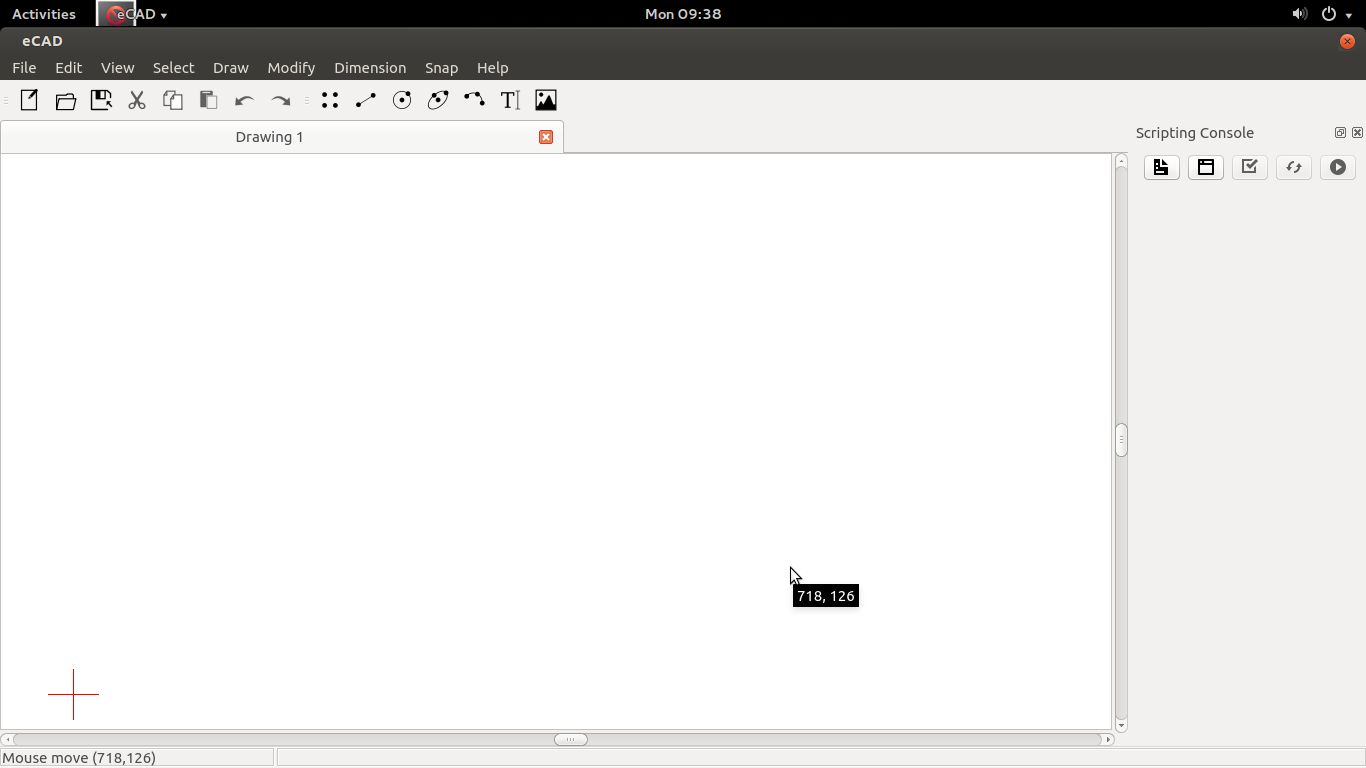
\includegraphics[width=0.7\textwidth]{images/togglegrig.png}\\
Go to View then Toolbars and check the command console it will be visible. By default command console is unchecked
\end{figure}
\newpage
\item \textbf{Status Bar}:
\begin{figure}[h!]
\centering
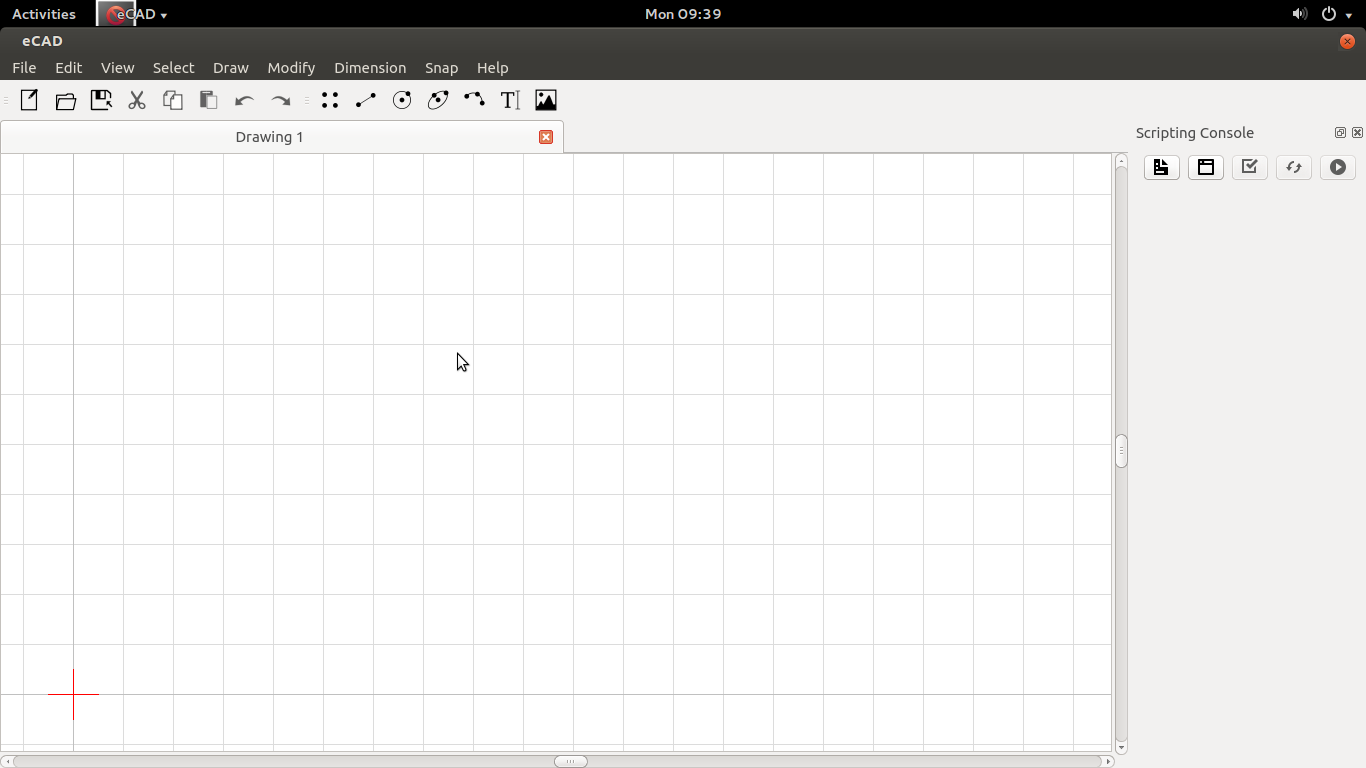
\includegraphics[width=0.7\textwidth]{images/togglestatus.png}\\
Go to View and uncheck the status bar the status bar will not be visible
\end{figure}
\item \textbf{Tool Bar}:
\begin{figure}[h!]
\centering
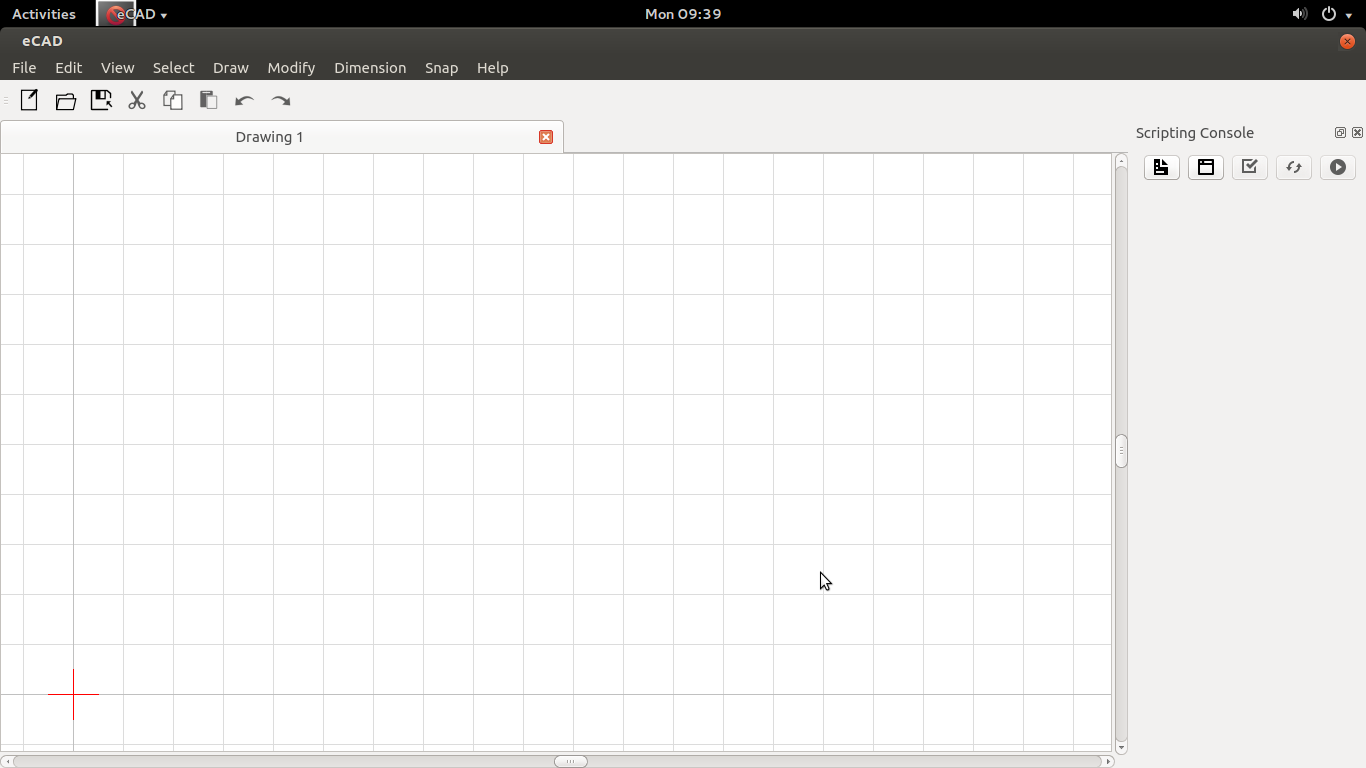
\includegraphics[width=0.7\textwidth]{images/toggletool.png}\\
Go to View then Toolbars and uncheck the toolbar the standard toolbar which contains all the entities will not be visible.
\end{figure}
\end{enumerate}